
\documentclass{standalone}
\usepackage{tikz}
\begin{document}
\begin{array}{cc}
\text{A} & \text{B} \\
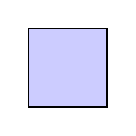
\begin{tikzpicture}
\draw[fill = blue!20, rotate = 90] (0,0) -- (1,0) -- (1,1) -- (0,1) -- cycle;
\end{tikzpicture} &
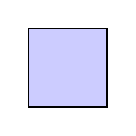
\begin{tikzpicture}
\draw[fill = blue!20, rotate = 180] (0,0) -- (1,0) -- (1,1) -- (0,1) -- cycle;
\end{tikzpicture} \\
\text{C} & \text{D} \\
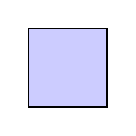
\begin{tikzpicture}
\draw[fill = blue!20, rotate = 270] (0,0) -- (1,0) -- (1,1) -- (0,1) -- cycle;
\end{tikzpicture} &
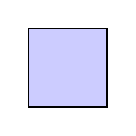
\begin{tikzpicture}
\draw[fill = blue!20, rotate = 360] (0,0) -- (1,0) -- (1,1) -- (0,1) -- cycle;
\end{tikzpicture}
\end{array}
\end{document}
